% Created 2024-10-25 vie 16:21
% Intended LaTeX compiler: pdflatex
\documentclass[10pt]{article}
\usepackage[utf8]{inputenc}
\usepackage{lmodern}
\usepackage[T1]{fontenc}
\usepackage[top=1in, bottom=1.in, left=1in, right=1in]{geometry}
\usepackage{graphicx}
\usepackage{longtable}
\usepackage{float}
\usepackage{wrapfig}
\usepackage{rotating}
\usepackage[normalem]{ulem}
\usepackage{amsmath}
\usepackage{textcomp}
\usepackage{marvosym}
\usepackage{wasysym}
\usepackage{amssymb}
\usepackage{amsmath}
\usepackage[theorems, skins]{tcolorbox}
\usepackage[version=3]{mhchem}
\usepackage[numbers,super,sort&compress]{natbib}
\usepackage{natmove}
\usepackage{url}
\usepackage[cache=false]{minted}
\usepackage[strings]{underscore}
\usepackage[linktocpage,pdfstartview=FitH,colorlinks,
linkcolor=blue,anchorcolor=blue,
citecolor=blue,filecolor=blue,menucolor=blue,urlcolor=blue]{hyperref}
\usepackage{attachfile}
\usepackage{setspace}
\usepackage[spanish, ]{babel}
\date{}
\title{Mortalidad y matrimonio en Inglaterra 1866--1911}
\begin{document}

\maketitle
\section*{Los datos}
\label{sec:org330bb23}

Los datos de este ejercicio corresponden a la mortalidad anual y la
proporción de matrimonios eclesiásticos en Inglaterra entre 1866 y
1911 

\textbf{Fuente:} Ejercicio proporcionado por el Prof. Miguel Jerez

\begin{description}
\item[{\texttt{Std\_mortality}}] Mortalidad anual por cada 1000 personas. Serie estandarizada.
\item[{\texttt{Proportion\_marriages}}] Proporción de matrimonios eclesiásticos
anuales por cada 1000 personas.
\item[{\texttt{d\_Std\_mortality}}] Primera diferencia de \texttt{Std\_mortality}.
\item[{\texttt{d\_Proportion\_marriages}}] Primera diferencia de
\texttt{Proportion\_marriages}.
\end{description}

\begin{minted}[frame=lines,fontsize=\scriptsize,linenos=]{r}
open mortality-marriages.gdt
\end{minted}

\begin{itemize}
\item Ficheros \url{https://github.com/mbujosab/EconometriaAplicada-SRC/tree/main/Ejercicios}
\begin{itemize}
\item Versión en \href{https://github.com/mbujosab/EconometriaAplicada-SRC/blob/main/Ejercicios/mortality-marriages.pdf}{pdf}
\item Datos: \href{mortality-marriages.gdt}{mortality-marriages.gdt}
\item Guión de gretl: \href{mortality-marriages.inp}{mortality-marriages.inp}
\end{itemize}
\end{itemize}
\section*{Datos en nivel de la serie de mortalidad}
\label{sec:org96737d7}

\subsection*{Gráfico de la serie temporal y su correlograma}
\label{sec:org8cb990d}

\begin{minted}[frame=lines,fontsize=\scriptsize,linenos=]{r}
gnuplot Std_mortality --time-series --with-lines --output="mortality.png"
corrgm Std_mortality 9 --plot="mortalityACF-PACF.png"
\end{minted}


\begin{center}
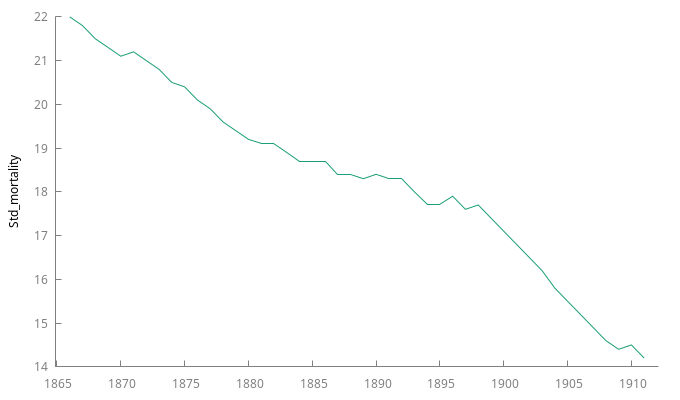
\includegraphics[width=0.5\textwidth]{./mortality-marriages/mortality.png} 
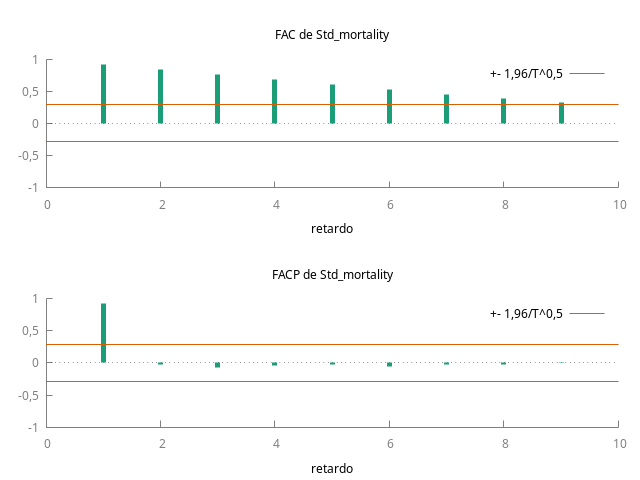
\includegraphics[width=0.4\textwidth]{./mortality-marriages/mortalityACF-PACF.png} 
\end{center}
\subsection*{Estimación de un modelo univariante para la serie de mortalidad}
\label{sec:org1fd8471}

\begin{minted}[frame=lines,fontsize=\scriptsize,linenos=]{r}
arima 1 0 2 ; Std_mortality
\end{minted}


\begin{verbatim}
Evaluaciones de la función: 289
Evaluaciones del gradiente: 80

Modelo 2: ARMA, usando las observaciones 1866-1911 (T = 46)
Estimado usando AS 197 (MV exacta)
Variable dependiente: Std_mortality
Desviaciones típicas basadas en el Hessiano

             coeficiente   Desv. típica      z      valor p 
  ----------------------------------------------------------
  const       18,0782       3,69647         4,891   1,00e-06 ***
  phi_1        0,996455     0,00501938    198,5     0,0000   ***
  theta_1      0,401166     0,171108        2,345   0,0191   **
  theta_2      0,345176     0,108887        3,170   0,0015   ***

Media de la vble. dep.  18,32174   D.T. de la vble. dep.   2,135615
Media de innovaciones  -0,094657   D.T. innovaciones       0,185241
R-cuadrado              0,994379   R-cuadrado corregido    0,994117
Log-verosimilitud       9,085184   Criterio de Akaike     -8,170368
Criterio de Schwarz     0,972839   Crit. de Hannan-Quinn  -4,745268

                       Real Imaginaria     Módulo Frecuencia
  -----------------------------------------------------------
  AR
   Raíz  1           1,0036     0,0000     1,0036     0,0000
  MA
   Raíz  1          -0,5811    -1,5998     1,7021    -0,3055
   Raíz  2          -0,5811     1,5998     1,7021     0,3055
  -----------------------------------------------------------
\end{verbatim}
\section*{Contraste de cointegración}
\label{sec:orge3af434}

\begin{minted}[frame=lines,fontsize=\scriptsize,linenos=]{r}
coint 9 Std_mortality Proportion_marriages --test-down
\end{minted}

\begin{verbatim}
Etapa 1: contrastando la existencia de una raíz unitaria en Std_mortality

Contraste aumentado de Dickey-Fuller para Std_mortality
contrastar hacia abajo desde 9 retardos, con el criterio AIC
tamaño muestral 45
la hipótesis nula de raíz unitaria es: [a = 1]

  contraste con constante 
  incluyendo 0 retardos de (1-L)Std_mortality
  modelo: (1-L)y = b0 + (a-1)*y(-1) + e
  valor estimado de (a - 1): 0,00678121
  estadístico de contraste: tau_c(1) = 0,615887
  valor p asintótico 0,9902
  Coef. de autocorrelación de primer orden de e: 0,085

Etapa 2: contrastando la existencia de una raíz unitaria en Proportion_marriages

Contraste aumentado de Dickey-Fuller para Proportion_marriages
contrastar hacia abajo desde 9 retardos, con el criterio AIC
tamaño muestral 39
la hipótesis nula de raíz unitaria es: [a = 1]

  contraste con constante 
  incluyendo 6 retardos de (1-L)Proportion_marriages
  modelo: (1-L)y = b0 + (a-1)*y(-1) + ... + e
  valor estimado de (a - 1): 0,0831149
  estadístico de contraste: tau_c(1) = 1,04236
  valor p asintótico 0,9971
  Coef. de autocorrelación de primer orden de e: -0,068
  diferencias retardadas: F(6, 31) = 3,197 [0,0147]

Etapa 3: regresión cointegrante

Regresión cointegrante - 
MCO, usando las observaciones 1866-1911 (T = 46)
Variable dependiente: Std_mortality

                      coeficiente  Desv. típica  Estadístico t  valor p 
  ----------------------------------------------------------------------
  const               -10,8466      1,42447         -7,614      1,45e-09 ***
  Proportion_marri~     0,418536    0,0203914       20,53       3,67e-24 ***

Media de la vble. dep.  18,32174   D.T. de la vble. dep.   2,135615
Suma de cuad. residuos  19,40865   D.T. de la regresión    0,664158
R-cuadrado              0,905434   R-cuadrado corregido    0,903284
Log-verosimilitud      -45,42395   Criterio de Akaike      94,84790
Criterio de Schwarz     98,50518   Crit. de Hannan-Quinn   96,21794
rho                     0,228283   Durbin-Watson           1,535570

Etapa 4: contrastando la existencia de una raíz unitaria en uhat

Contraste aumentado de Dickey-Fuller para uhat
contrastar hacia abajo desde 9 retardos, con el criterio AIC
tamaño muestral 45
la hipótesis nula de raíz unitaria es: [a = 1]

  contraste sin constante 
  incluyendo 0 retardos de (1-L)uhat
  modelo: (1-L)y = (a-1)*y(-1) + e
  valor estimado de (a - 1): -0,771717
  estadístico de contraste: tau_c(2) = -5,22784
  valor p asintótico 5,236e-05
  Coef. de autocorrelación de primer orden de e: 0,023

Hay evidencia de una relación cointegrante si:
(a) La hipótesis de existencia de raíz unitaria no se rechaza para las variables individuales y
(b) La hipótesis de existencia de raíz unitaria se rechaza para los residuos (uhat) de la regresión cointegrante.
\end{verbatim}
\section*{Regresión de la mortalidad sobre la proporción de matrimonios eclesiásticos}
\label{sec:org49b1fb0}

\begin{minted}[frame=lines,fontsize=\scriptsize,linenos=]{r}
ols Std_mortality 0 Proportion_marriages
modtest --normality --quiet
modtest --white --quiet
modtest --autocorr 5 --quiet
\end{minted}

\begin{verbatim}
Modelo 6: MCO, usando las observaciones 1866-1911 (T = 46)
Variable dependiente: Std_mortality

                      coeficiente  Desv. típica  Estadístico t  valor p 
  ----------------------------------------------------------------------
  const               -10,8466      1,42447         -7,614      1,45e-09 ***
  Proportion_marri~     0,418536    0,0203914       20,53       3,67e-24 ***

Media de la vble. dep.  18,32174   D.T. de la vble. dep.   2,135615
Suma de cuad. residuos  19,40865   D.T. de la regresión    0,664158
R-cuadrado              0,905434   R-cuadrado corregido    0,903284
F(1, 44)                421,2815   Valor p (de F)          3,67e-24
Log-verosimilitud      -45,42395   Criterio de Akaike      94,84790
Criterio de Schwarz     98,50518   Crit. de Hannan-Quinn   96,21794
rho                     0,228283   Durbin-Watson           1,535570


Contraste de la hipótesis nula de distribución Normal:
Chi-cuadrado(2) = 0,260 con valor p 0,87796


Contraste de heterocedasticidad de White

Estadístico de contraste: TR^2 = 1,729996,
con valor p = P(Chi-cuadrado(2) > 1,729996) = 0,421052


Contraste de Breusch-Godfrey para autocorrelación hasta el orden 5

Estadístico de contraste: LMF = 1,947454,
con valor p = P(F(5,39) > 1,94745) = 0,108

Estadístico alternativo: TR^2 = 9,190388,
con valor p = P(Chi-cuadrado(5) > 9,19039) = 0,102

Ljung-Box Q' = 9,05845,
con valor p = P(Chi-cuadrado(5) > 9,05845) = 0,107
\end{verbatim}
\section*{Regresión en primeras diferencias}
\label{sec:orga91617c}

\begin{minted}[frame=lines,fontsize=\scriptsize,linenos=]{r}
diff Std_mortality Proportion_marriages
ols d_Std_mortality 0 d_Proportion_marriages
modtest --normality --quiet
modtest --white --quiet
modtest --autocorr 5 --quiet
\end{minted}

\begin{verbatim}
Modelo 8: MCO, usando las observaciones 1867-1911 (T = 45)
Variable dependiente: d_Std_mortality

                      coeficiente  Desv. típica  Estadístico t  valor p 
  ----------------------------------------------------------------------
  const               -0,172792     0,0230316       -7,502      2,43e-09 ***
  d_Proportion_mar~    0,00142536   0,0117781        0,1210     0,9042  

Media de la vble. dep. -0,173333   D.T. de la vble. dep.   0,149848
Suma de cuad. residuos  0,987664   D.T. de la regresión    0,151555
R-cuadrado              0,000340   R-cuadrado corregido   -0,022907
F(1, 43)                0,014645   Valor p (de F)          0,904241
Log-verosimilitud       22,07697   Criterio de Akaike     -40,15393
Criterio de Schwarz    -36,54061   Crit. de Hannan-Quinn  -38,80692
rho                     0,089193   Durbin-Watson           1,806988


Contraste de la hipótesis nula de distribución Normal:
Chi-cuadrado(2) = 14,808 con valor p 0,00061


Contraste de heterocedasticidad de White

Estadístico de contraste: TR^2 = 2,149006,
con valor p = P(Chi-cuadrado(2) > 2,149006) = 0,341467


Contraste de Breusch-Godfrey para autocorrelación hasta el orden 5

Estadístico de contraste: LMF = 0,589588,
con valor p = P(F(5,38) > 0,589588) = 0,708

Estadístico alternativo: TR^2 = 3,239657,
con valor p = P(Chi-cuadrado(5) > 3,23966) = 0,663

Ljung-Box Q' = 4,0454,
con valor p = P(Chi-cuadrado(5) > 4,0454) = 0,543
\end{verbatim}
\section*{Preguntas}
\label{sec:orgb2fcf5d}

\subsection*{Pregunta 1}
\label{sec:org062b603}

Discuta de todas las formas posibles si la serie temporal de
mortalidad (\texttt{Std\_mortality}) es estacionaria en media (i.e., la
realización de un proceso estocástico estacionario), usando para ello
los resultados de los apartados \hyperref[sec:org96737d7]{Datos en nivel de la serie de mortalidad} y \hyperref[sec:orge3af434]{Contraste de cointegración}.

(\hyperref[sec:orga891e51]{Respuesta 1})
\subsection*{Pregunta 2}
\label{sec:org17dfe6a}

Discuta si las series de mortalidad y proporción de matrimonios
eclesiásticos están cointegradas, a partir de los resultados del
apartado \hyperref[sec:orge3af434]{Contraste de cointegración}.

(\hyperref[sec:org12b080a]{Respuesta 2})
\subsection*{Pregunta 3}
\label{sec:org94733fd}

Sin embargo, ¿qué sugieren los resultados de las secciones \hyperref[sec:org49b1fb0]{Regresión de la mortalidad sobre la proporción de matrimonios eclesiásticos} y
\hyperref[sec:orga91617c]{Regresión en primeras diferencias} respecto a la relación entre
\texttt{Std\_mortality} y \texttt{Proportion\_marriages}?

(\hyperref[sec:orge9130b5]{Respuesta 3})
\subsection*{Pregunta 4}
\label{sec:org267f7db}

Los listados en \hyperref[sec:org49b1fb0]{Regresión de la mortalidad sobre la proporción de matrimonios eclesiásticos} y \hyperref[sec:orga91617c]{Regresión en primeras diferencias} muestran
los principales resultados obtenidos al estimar por MCO dos modelos de
regresión que relacionan las dos variables consideradas en este
ejercicio. Resuma y comente los resultados de estimación y diagnosis
que le parezcan más relevantes. Si detecta alguna desviación del
cumplimiento de las hipótesis habituales, discuta sus consecuencias
sobre las propiedades del estimador MCO y sugiera una forma de
tratarla.

(\hyperref[sec:org39869ab]{Respuesta 4})
\subsection*{Pregunta 5}
\label{sec:org6ceee13}

Interprete la pendiente de la regresión cointegrante estimada en la
Etapa 3 del \hyperref[sec:orge3af434]{Contraste de cointegración}.

(\hyperref[sec:orgec5905c]{Respuesta 5})
\subsection*{Pregunta 6}
\label{sec:org311cdee}

Indique cuáles de las siguientes expresiones representan el modelo de
la sección \hyperref[sec:org1fd8471]{Estimación de un modelo univariante para la serie de mortalidad}, con un redondeo a tres decimales 

\begin{enumerate}
\item \(\left( 1 - 0.997 \, \mathsf{B} \right) \, \left(X_t - 18.078 \right) = \left( 1 + 0.401 \, \mathsf{B} + 0.345 \, \mathsf{B}^2 \right) \hat U_t\)
\item \(\left( 1 - 0.997 \, \mathsf{B} \right) \, \left(X_t - 18.078 \right) = \left( 1 - 0.401 \, \mathsf{B}  - 0.345 \, \mathsf{B}^2 \right) \hat U_t\)
\item \(\left( 1 + 0.997 \, \mathsf{B} \right) \, \left(X_t - 18.078 \right) = \left( 1 + 0.401 \, \mathsf{B}  + 0.345 \, \mathsf{B}^2 \right) \hat U_t\)
\item \(\,{X_t} = 18.078 + \frac{  1 + 0.401 \, \mathsf{B}  + 0.345 \, \mathsf{B}^2 }{ 1 - 0.997 \, \mathsf{B} } \hat U_t\)
\item \(\,{X_t} = -18.078 + \frac{  1 + 0.401 \, \mathsf{B}  + 0.345 \, \mathsf{B}^2 }{ 1 - 0.997 \, \mathsf{B} } \hat U_t\)
\item \(\,{X_t} = 18.078 + \frac{  1 - 0.401 \, \mathsf{B} - 0.345 \, \mathsf{B}^2 }{ 1 - 0.997 \, \mathsf{B} } \hat U_t\)
\item \(\,{X_t} = 18.078 + \frac{  1 + 0.401 \, \mathsf{B}  + 0.345 \, \mathsf{B}^2 }{ 1 + 0.997 \, \mathsf{B} } \hat U_t\)
\item \(\frac{ 1 - 0.997 \, \mathsf{B} }{1 + 0.401 \, \mathsf{B}  + 0.345 \, \mathsf{B}^2 } \, \left(X_t - 18.078 \right)=  \hat U_t\)
\item \(\frac{ 1 - 0.997 \, \mathsf{B} }{1 + 0.401 \, \mathsf{B}  + 0.345 \, \mathsf{B}^2 } \, X_t = 18.078 + \hat U_t\)
\item \(\frac{ 1 - 0.997 \, \mathsf{B} }{1 - 0.401 \, \mathsf{B} - 0.345 \, \mathsf{B}^2 } \, \left(X_t - 18.078 \right)=  \hat U_t\)
\end{enumerate}

(\hyperref[sec:orgb8d29e5]{Respuesta 6})
\subsection*{Pregunta 7}
\label{sec:orgb3917d4}

A la luz de la \hyperref[sec:org1fd8471]{Estimación de un modelo univariante para la serie de mortalidad}, si tuviera que clasificar el proceso estocástico
subyacente del que la serie temporal es una realización ¿diría que es
invertible?  ¿O que no lo es?  ¿diría que es estacionario? ¿O que no
lo es? Explique su respuesta.

(\hyperref[sec:orgbb37eae]{Respuesta 7})
\subsection*{Pregunta 8}
\label{sec:org1275d33}

¿Cuáles de los modelos de más arriba considera aceptables? ¿O qué
mejoras sugeriría para ellos?

(\hyperref[sec:orgec7dc4d]{Respuesta 8})

\newpage
\section*{Respuestas}
\label{sec:orgd13a142}

\subsection*{Respuesta 1}
\label{sec:orga891e51}

La serie temporal \texttt{Std\_mortality} NO es estacionaria en media, como se
aprecia en las secciones:
\begin{itemize}
\item \hyperref[sec:org8cb990d]{Gráfico de la serie temporal y su correlograma}. 
\begin{itemize}
\item El gráfico de la serie muestra una tendencia decreciente.
\item La FAC muestra mucha persistencia, los coeficientes decrecen a un
ritmo aproximadamente lineal; y el primer coeficiente de la PACF
está próximo a uno.
\end{itemize}
\item \hyperref[sec:org1fd8471]{Estimación de un modelo univariante para la serie de mortalidad}: El
modelo univariante estimado tiene una raíz AR aproximadamente igual
a \(1\).
\item \hyperref[sec:orge3af434]{Contraste de cointegración}: El test ADF calculado en la Etapa 1 no
rechaza la hipótesis (raíz unitaria) con un p-valor de \texttt{0.9902}
\end{itemize}

(\hyperref[sec:org062b603]{Pregunta 1})
\subsection*{Respuesta 2}
\label{sec:org12b080a}

Las conclusiones de las distintas etapas del test de cointegración son los siguientes:
\begin{description}
\item[{Etapa 1}] El test ADF no rechaza que la serie de mortalidad sea
I(1). \texttt{(valor p asintótico 0,9902)}
\item[{Etapa 2}] El test ADF no rechaza que la serie de proporción de
matrimonios eclesiásticos sea I(1). \texttt{(valor p asintótico 0,9971)}
\item[{Etapa 3}] La regresión (cointegrante) de mortalidad sobre la
proporción de matrimonios eclesiásticos es significativa (parámetros
significativos y elevado \(R^2\) \texttt{(0,905434)}.
\item[{Etapa 4}] El test ADF rechaza contundentemente que los residuos de
la regresión cointegrante sean I(1). \texttt{(valor p asintótico
  5,236e-05)}
\end{description}

Consecuentemente, el test indica que ambas series están cointegradas
(\emph{pero, como sugiere tanto el sentido común como la \hyperref[sec:orga91617c]{Regresión en primeras diferencias} la relación es espuria}, véase la pregunta 3).

(\hyperref[sec:org17dfe6a]{Pregunta 2})
\subsection*{Respuesta 3}
\label{sec:orge9130b5}

Aunque el modelo de \hyperref[sec:org49b1fb0]{Regresión de la mortalidad sobre la proporción de matrimonios eclesiásticos} muestra un buen ajuste (un elevado \(R^2\)) y
los parámetros estimados son muy significativos, la relación entre
ambas variables se desvanece al diferenciar los datos para lograr la
estacionariedad. Ello sugiere, al igual que el sentido común, que \uline{la
relación es espuria}.

(\hyperref[sec:org94733fd]{Pregunta 3})
\subsection*{Respuesta 4}
\label{sec:org39869ab}

\begin{description}
\item[{Modelo de regresión MCO para datos en nivel}] (\hyperref[sec:org49b1fb0]{Regresión de la mortalidad sobre la proporción de matrimonios eclesiásticos}): Todos
los coeficientes son muy significativos. El ajuste del modelo,
medido por el valor del \(R^2\) es muy elevado. Los contrastes sobre
los residuos no rechazan (ni al 1\%, ni al 5\% ni al 10\% de
significación) las hipótesis nulas de normalidad, homoscedasticidad
y ausencia de autocorrelación. Es decir, de la salida de Gretl no se
puede inferir que haya ningún problema con este modelo.

\item[{Modelo para datos en primeras diferencias}] (\hyperref[sec:orga91617c]{Regresión en primeras diferencias}): El único coeficiente significativo es el término
constante. El ajuste del modelo, medido por el valor del \(R^2\), es
prácticamente nulo. Los contrastes residuales rechazan la hipótesis
nula de normalidad, aunque no rechazan las de homoscedasticidad y
ausencia de autocorrelación. 

Si las perturbaciones no tienen distribución normal las estimaciones
no serán eficientes en el sentido máximo-verosímil (aunque sí en el
de Gauss-Markov) y la distribución de los estadísticos habituales
será distinta de la teórica bajo el supuesto de normalidad de las
perturbaciones (por ejemplo, los estadísticos de la \(t\) no tendrán
exactamente una distribución \emph{t} de student).

No obstante, dado que la relación entre variables es espuria,
ninguno de estos modelos de regresión es válido como explicación de
la tasa de mortalidad.
\end{description}

(\hyperref[sec:org267f7db]{Pregunta 4})
\subsection*{Respuesta 5}
\label{sec:orgec5905c}

La pendiente de la regresión estimada en la Etapa 3 (que es la misma
que la de la sección de la regresión en niveles) indica que un aumento
de un uno por mil en la proporción de matrimonios eclesiásticos da
lugar a un aumento de un 0.419 por mil en la mortalidad esperada
(pero, dado que la relación es espuria, interpretar este resultado
carece de sentido).

(\hyperref[sec:org6ceee13]{Pregunta 5})
\subsection*{Respuesta 6}
\label{sec:orgb8d29e5}

Recuerde que signo de los parámetros MA en las salidas de Gretl tienen
el signo cambiado respecto a convenio habitual en los manuales de
series temporales, es decir, para los polinomios AR
\((1-\phi_1\mathsf{B}-\cdots-\phi_p\mathsf{B}^p)\), tenemos que \texttt{phi\_j}
es "\(\phi_j\)" (es decir, al escribir el modelo el signo del parámetro
\texttt{phi\_j} aparece con un menos delante); pero para los MA
\((1-\theta_1\mathsf{B}-\cdots-\theta_p\mathsf{B}^p)\), tenemos que
\texttt{theta\_j} es "\(-\theta_j\)" (es decir, al escribir no cambiamos el
signo de parámetro \texttt{theta\_j} pues ya lleva el "\(-\)" incorporado).
Además, \texttt{const} es la estimación del valor esperado \(\mu\) del proceso
\(\boldsymbol{X}\), es decir, que \((X_t-\mu\mid t\in\mathbb{Z})\) es un
proceso ARMA de media cero.

Por tanto, las expresiones correctas son:

\begin{description}
\item[{Expresión 1}] modelo ARMA(\(1,2\)): \(\;\boldsymbol{\phi}(\mathsf{B})({X_t}-\mu)=\boldsymbol{\theta}(\mathsf{B}){U_t}\)
\item[{Expresión 4}] su representación MA(\(\infty\)): \(\;({X_t}-\mu)=\frac{\boldsymbol{\theta}}{\boldsymbol{\phi}}(\mathsf{B}){U_t}\;\rightarrow\;{X_t}=\mu+\frac{\boldsymbol{\theta}}{\boldsymbol{\phi}}(\mathsf{B}){U_t}\)
\item[{Expresión 8}] su representación AR(\(\infty\)): \(\;\frac{\boldsymbol{\phi}}{\boldsymbol{\theta}}(\mathsf{B})({X_t}-\mu)={U_t}\)
\end{description}

¡Ojo, la cuarta expresión solo es posible porque \(\phi_1\) no es
exactamente 1! Si fuera 1, el polinomio autorregresivo \(1-\mathsf{B}\)
no tendría una inversa sumable y, por tanto, ni el proceso sería
estacionario, ni habría una representación del proceso como media
móvil infinita como la Expresión 4.


(\hyperref[sec:org311cdee]{Pregunta 6})
\subsection*{Respuesta 7}
\label{sec:orgbb37eae}

La raíz AR estimada está muy próxima a 1, por lo que cabe pensar que
la serie proviene de un proceso estocástico NO estacionario. Sin
embargo, las raíces del polinomio MA tienen un módulo claramente mayor
que uno, por lo que el modelo tiene claramente una representación
AR(\(\infty\)), es decir, es invertible.

(\hyperref[sec:orgb3917d4]{Pregunta 7})
\subsection*{Respuesta 8}
\label{sec:orgec7dc4d}

¿Cuáles de los modelos de más arriba considera aceptables? ¿O qué
mejoras sugeriría para ellos?

\begin{description}
\item[{En cuanto al modelo univariante}] Probablemente debería incorporar
una diferencia ordinaria, en lugar de un término AR(1).

\item[{En cuanto a los modelos de regresión}] En el modelo de las serie en
diferencias hay, probablemente, un problema de autocorrelación dado
el elevado valor del estadístico Durbin-Watson (es próximo a 2), por
lo que quizá debería ser estimado por mínimos cuadrados
generalizados asumiendo un modelo autorregresivo AR(1) para el
error.

No obstante, el modelo en diferencias (y el sentido común) sugiere
que la relación entre ambas variables es espuria. Consecuentemente,
ninguna de las dos regresiones (en niveles o en diferencias)
arrojará un modelo aceptable ni siquiera con las mejoras sugeridas.
\end{description}

(\hyperref[sec:org1275d33]{Pregunta 8})
\end{document}
